% Dynamic Block Timing Diagram
% Shows relationship between utilization, block time, and emission
%
% ACCESSIBILITY ALT TEXT:
% A dual-axis graph showing dynamic block timing. X-axis shows network
% utilization (0-100%). Left Y-axis shows block time in seconds (5-40s),
% with a blue descending line from 40s at idle to 5s at full utilization.
% Right Y-axis shows blocks per hour (90-720), with an orange dashed curve
% rising inversely. Three colored regions indicate low (green), moderate
% (yellow), and high (red) usage zones. Formula shown: T = Tmin + (Tmax -
% Tmin) * (1 - U). Key insight: low usage means slower blocks and less
% emission; high usage means faster blocks and more throughput.

\begin{figure}[ht]
\centering
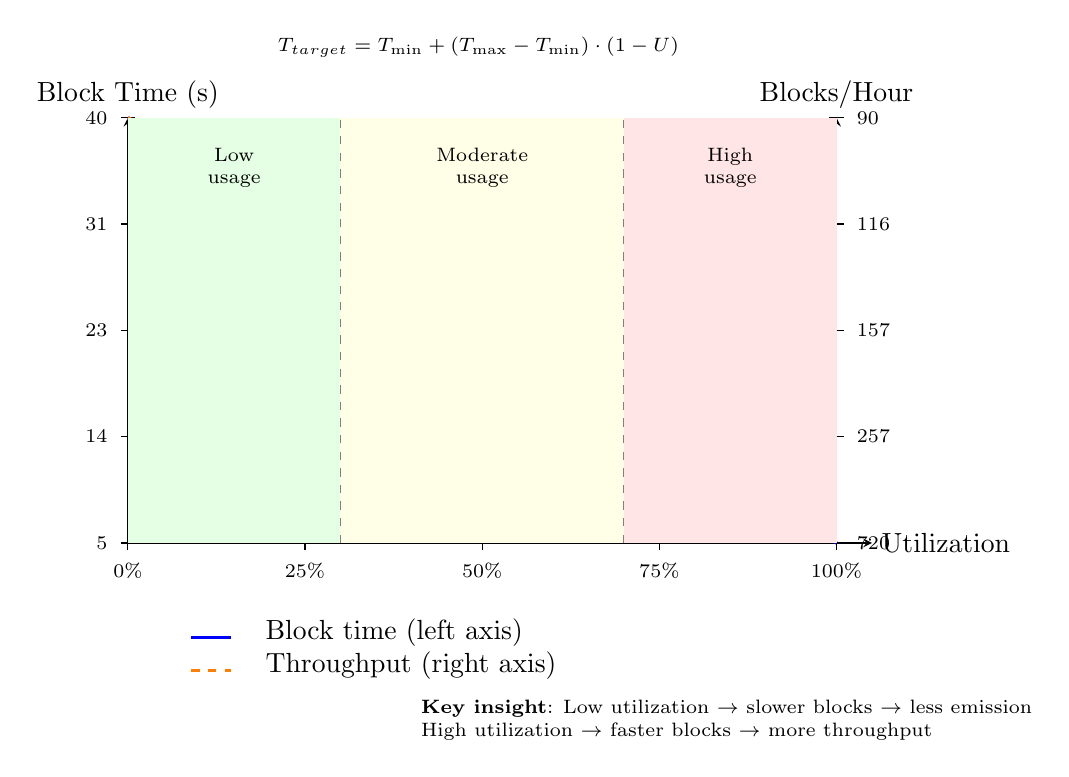
\begin{tikzpicture}[
    scale=0.9,
    >=stealth,
]

% Main axes
\draw[->] (0,0) -- (10.5,0) node[right] {Utilization};
\draw[->] (0,0) -- (0,6) node[above] {Block Time (s)};

% Secondary Y-axis (right side) for emission
\draw[->] (10,0) -- (10,6) node[above] {Blocks/Hour};

% X-axis labels
\foreach \x/\label in {0/0\%, 2.5/25\%, 5/50\%, 7.5/75\%, 10/100\%} {
    \draw (\x,-0.1) -- (\x,0.1);
    \node[below] at (\x,-0.15) {\scriptsize \label};
}

% Left Y-axis labels (block time: 5s to 40s)
\foreach \y/\label in {0/5, 1.5/14, 3/23, 4.5/31, 6/40} {
    \draw (-0.1,\y) -- (0.1,\y);
    \node[left] at (-0.15,\y) {\scriptsize \label};
}

% Right Y-axis labels (blocks per hour)
\foreach \y/\label in {0/720, 1.5/257, 3/157, 4.5/116, 6/90} {
    \draw (9.9,\y) -- (10.1,\y);
    \node[right] at (10.15,\y) {\scriptsize \label};
}

% Block time curve (linear: T = 40 - 35*U, mapped to y = 6 - 6*x/10)
\draw[very thick, blue] (0,6) -- (10,0);

% Blocks per hour curve (inverse relationship, approximately)
% At U=0: 40s -> 90 blocks/hr; At U=1: 5s -> 720 blocks/hr
\draw[very thick, orange, dashed]
    (0,6) .. controls (3,4.5) and (7,1.5) .. (10,0);

% Fill regions to show high/low utilization
\fill[green!10] (0,0) rectangle (3,6);
\fill[yellow!10] (3,0) rectangle (7,6);
\fill[red!10] (7,0) rectangle (10,6);

% Vertical region separators
\draw[dashed, gray] (3,0) -- (3,6);
\draw[dashed, gray] (7,0) -- (7,6);

% Region labels
\node[font=\scriptsize, align=center] at (1.5,5.3) {Low\\usage};
\node[font=\scriptsize, align=center] at (5,5.3) {Moderate\\usage};
\node[font=\scriptsize, align=center] at (8.5,5.3) {High\\usage};

% Legend
\node[anchor=west] at (0.5,-1.5) {
    \begin{tabular}{cl}
    \tikz\draw[very thick, blue] (0,0) -- (0.5,0); & Block time (left axis) \\
    \tikz\draw[very thick, orange, dashed] (0,0) -- (0.5,0); & Throughput (right axis) \\
    \end{tabular}
};

% Key insight annotation
\node[align=left, font=\scriptsize, anchor=west] at (4,-2.5) {
    \textbf{Key insight}: Low utilization $\rightarrow$ slower blocks $\rightarrow$ less emission\\
    High utilization $\rightarrow$ faster blocks $\rightarrow$ more throughput
};

% Formula
\node[align=center, font=\scriptsize] at (5,7) {
    $T_{\text{target}} = T_{\min} + (T_{\max} - T_{\min}) \cdot (1 - U)$
};

\end{tikzpicture}
\caption{Dynamic block timing mechanism. Block time varies linearly from 40
seconds (idle network) to 5 seconds (maximum demand). This creates natural
inflation dampening: low usage produces fewer blocks and less emission, while
high usage increases throughput to meet demand. The system self-regulates
based on mempool pressure.}
\label{fig:dynamic-timing}
\end{figure}
